\section{UML}

\subsection{Klassendiagram}
Ein \textbf{Klassendiagramm} beschreibt die statische Struktur eines Programms und spiegelt in abstrakter Form den Quellcode eines Programmes wider.
Wesentliche Einheiten sind Klassen und Schnittstellen und deren Beziehungen zueinander.
Der folgende Quellcode wird in Abbildung \ref{fig:cc-classdiagram} in die im Kurs verwendete UML-Notation überführt:

\begin{minted}[mathescape,
    linenos,
    numbersep=5pt,
    gobble=2,
    fontsize=\small]{java}
    class X {
        private I[] interfaces;
        public void M(Y y) {
        }
    }
    class Y {}
    interface I {}
    class A implements I {}
    class B implements I {}
    public class Main {
        public static void main(String... args) {
            B b = new B();
            X x = new X(new A())
        }
    }
\end{minted}

\begin{figure}
    \centering
    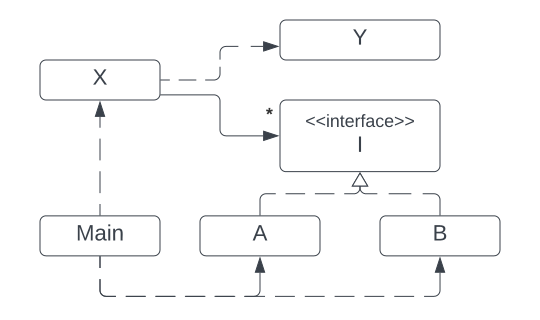
\includegraphics[scale=0.35]{chapters/Anhang/CheatSheet/img/classdiagram}
    \caption{Klassendiagramm (Quelle: eigene)}
    \label{fig:cc-classdiagram}
\end{figure}

\subsection{Objektdiagramm}
Ein \textbf{Objektdiagramm} beschreibt die Situation zu einem bestimmten Zeitpunkt während der Ausführung des Programms.\\

\subsection*{Notation}
Ein Objekt in einem Objektdiagramm wird durch einen führenden Doppelpunkt (dem ein Bezeichner vorangestellt werden kann) und dem Klassenname des Objektes dargestellt (\textbf{unterstrichen}).

\subsection{Sequenzdiagramm}
Ein \textbf{Sequenzdiagramm} dient zur Beschreibung des dynamischen Verhaltens eines Programms.
Es wird grafisch dargestellt, wie in einer bestimmten Situation  unter bestimmten Bedingungen welche Methoden welche anderen Methoden aufrufen, und auf welchen Objekten diese Methoden aufgerufen werden.\\

\subsection*{Notizen}
Erzeugt ein Methodenaufruf ein anderes Objekt, endet der \code{new()} Aufruf an dem Kästchen, das das Objekt repräsentiert.
Der Konstruktoraufruf wird über einen Balken, der direkt unter dem Kästchen folgt, dargestellt.
Der Sachverhalt wird mit Hilfe des folgenden Codes in Abbildung ~\ref{fig:cc-sequence} dargestellt\footnote{
    Aufruf der Methode \textit{x.m()} von einem externen Akteur der Einfachheit halber ausgelassen.
}:

\begin{minted}[mathescape,
    linenos,
    numbersep=5pt,
    gobble=2,
    fontsize=\small]{java}
    class X {
        public void m() {
            Y y = new Y();
        }
    }
\end{minted}

\begin{figure}
    \centering
    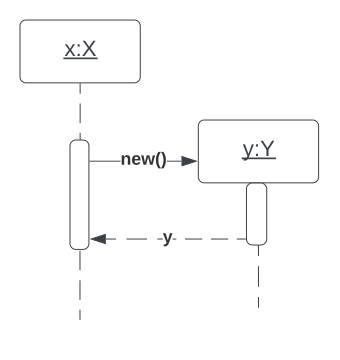
\includegraphics[scale=0.35]{chapters/Anhang/CheatSheet/img/constructor}
    \caption{Konstruktoraufruf als Sequenzdiagramm (Quelle: eigene)}
    \label{fig:cc-sequence}
\end{figure}
